\begin{center}
    

\tikzset{every picture/.style={line width=0.75pt}} %set default line width to 0.75pt        

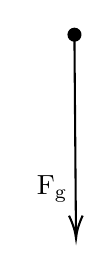
\begin{tikzpicture}[x=0.75pt,y=0.75pt,yscale=-1,xscale=1]
%uncomment if require: \path (0,300); %set diagram left start at 0, and has height of 300

%Shape: Circle [id:dp6401125961176861] 
\draw  [fill={rgb, 255:red, 0; green, 0; blue, 0 }  ,fill opacity=1 ] (330.88,127.88) .. controls (330.88,126.29) and (332.16,125) .. (333.75,125) .. controls (335.34,125) and (336.63,126.29) .. (336.63,127.88) .. controls (336.63,129.46) and (335.34,130.75) .. (333.75,130.75) .. controls (332.16,130.75) and (330.88,129.46) .. (330.88,127.88) -- cycle ;
%Straight Lines [id:da01700580379156591] 
\draw    (333.75,130.75) -- (334.48,224) ;
\draw [shift={(334.5,226)}, rotate = 269.55] [color={rgb, 255:red, 0; green, 0; blue, 0 }  ][line width=0.75]    (10.93,-3.29) .. controls (6.95,-1.4) and (3.31,-0.3) .. (0,0) .. controls (3.31,0.3) and (6.95,1.4) .. (10.93,3.29)   ;

% Text Node
\draw (323,202) node   [align=left] {F\textsubscript{g}};


\end{tikzpicture}

\end{center}